\section{Data Wastage by QUIC and TCP}

Let us look at the total data downloaded by QUIC and TCP and the data wasted by both the protocols. Data wasted is computed by considering the fact that if there is lower resolution data when a higher resolution is being played then the lower resolution data is being wasted. The amount of data downloaded and data wasted has been calculated using the bit rates available for each itag in the HAR files.

\begin{figure}[ht!]
    \centering
    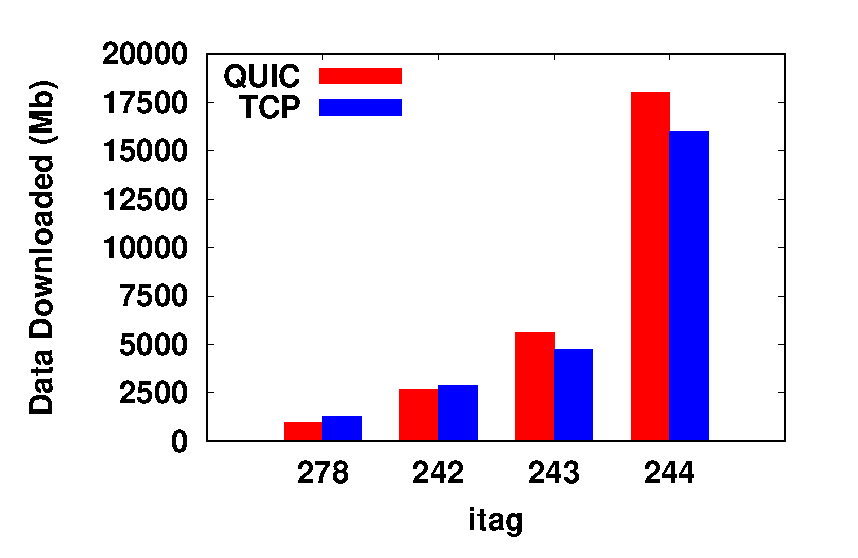
\includegraphics[width=0.9\linewidth]{img/CDF/Data_Dowloaded}
    \caption{Amount of Data Downloaded}
    \label{fig:rabuf761856q}
\end{figure}
%\clearpage
\begin{figure}[ht!]
    \centering
    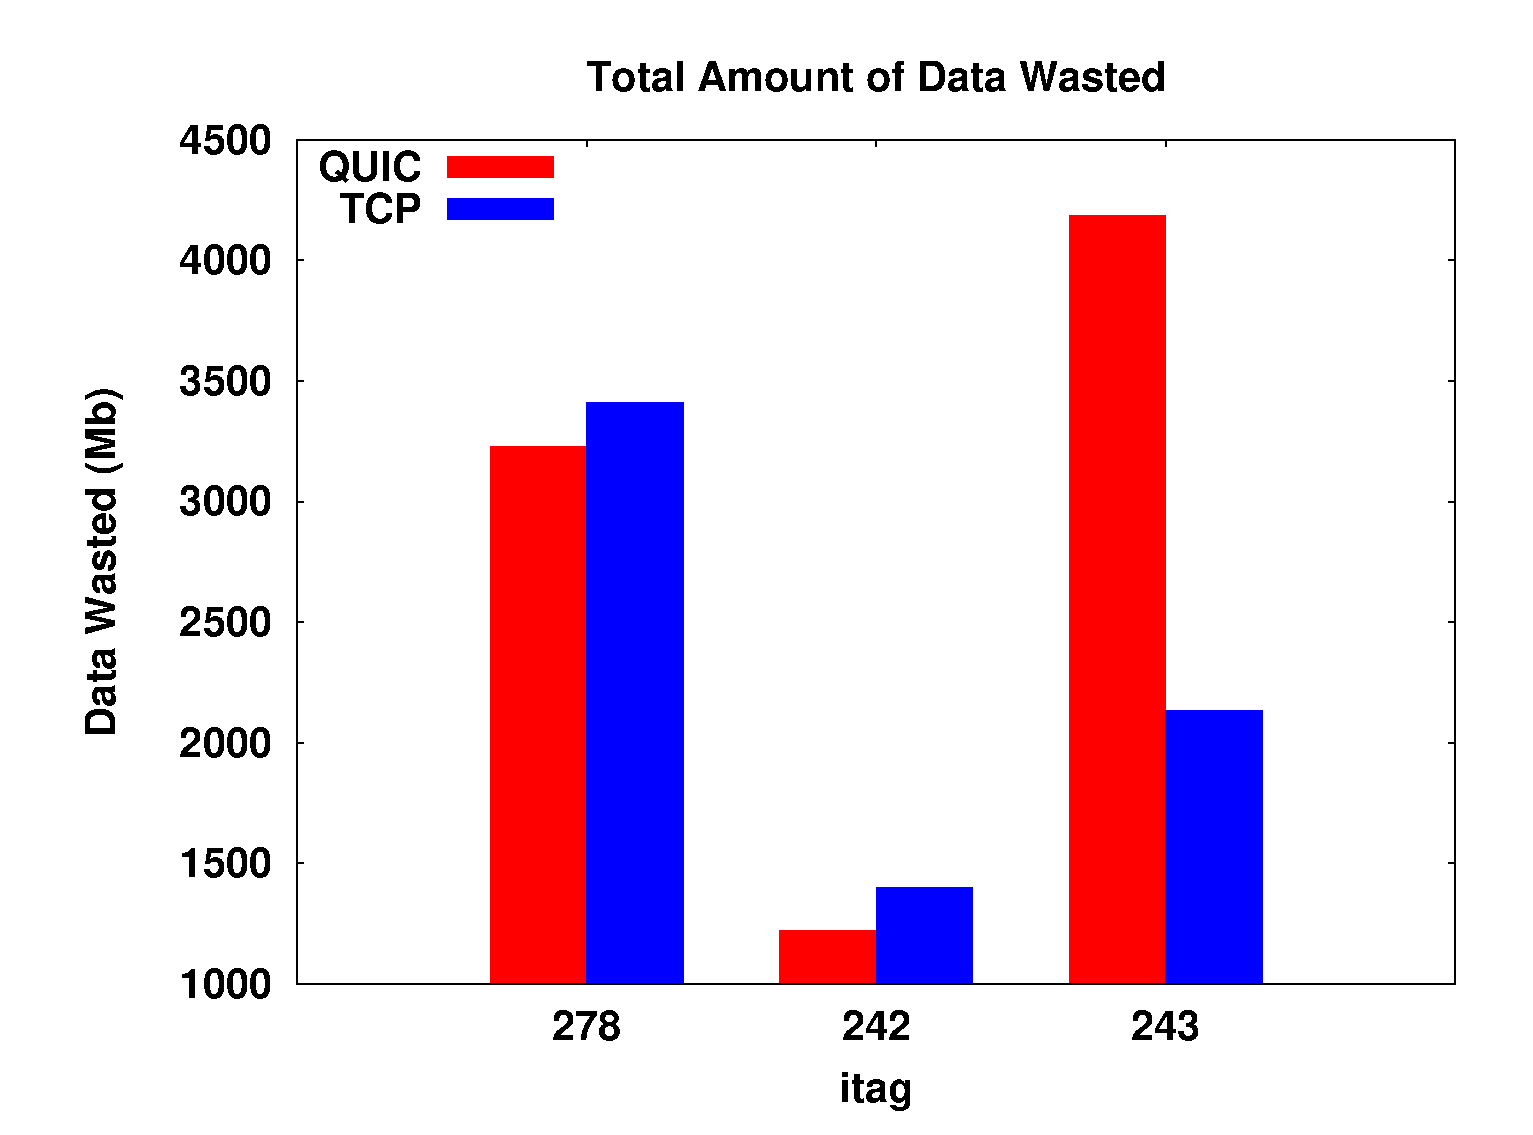
\includegraphics[width=0.9\linewidth]{img/CDF/DataWasted}
    \caption{Amount of Data Wasted}
    \label{fig:rabuf76q1}
\end{figure}

\begin{table}[ht!]
\centering
\scriptsize
\begin{tabular}{||c |c |c|c|c||} 
 \hline
 \textbf{Itag} & \textbf{Resolution} & \textbf{Downloaded (Mb)}& \textbf{Wasted (Mb)}& \textbf{\% Wasted }  \\ [0.5ex] 
 \hline\hline
  278 & 256x144 & 7669 & 3230 & 42.12\%\\ 
 \hline
  242 & 426x240 & 21232 & 1219 &5.74\%\\ 
 \hline
  243 & 640x360 & 44894 & 4187 &9.33\%\\ 
  \hline
  \hline
  Total &  & 73795 & 8636 &11.7\%\\ 
 \hline
\end{tabular}
\caption{Data Wastage for QUIC}
\label{table:3}
\end{table}

\begin{table}[ht!]
\centering
\scriptsize
\begin{tabular}{||c |c |c|c|c||} 
 \hline
 \textbf{Itag} & \textbf{Resolution} & \textbf{Downloaded (Mb)}& \textbf{Wasted (Mb)}& \textbf{\% Wasted }  \\ [0.5ex] 
 \hline\hline
  278 & 256x144 & 10049 & 3412 & 33.95\%\\ 
 \hline
  242 & 426x240 & 23028 & 1399 &6.07\%\\ 
 \hline
  243 & 640x360 & 37911 & 2134 &5.63\%\\ 
  \hline
  \hline
  Total &  & 70988 & 6945 &9.78\%\\ 
 \hline
\end{tabular}
\caption{Data Wastage for TCP}
\label{table:4}
\end{table}

\subsection{Number of Video Resolution Changes}
For each protocol we counted the number of times Video resolution has changed and categorized it into upward resolution changes and downward resolution changes. It should not be confused that TCP is performing better with TCP making more number of upward resolution changes because we also need to look at the total number of resolution changes ans the number of downward resolution changes. 

\begin{figure}[ht!] 
\centering
\begin{minipage}{0.48\linewidth}
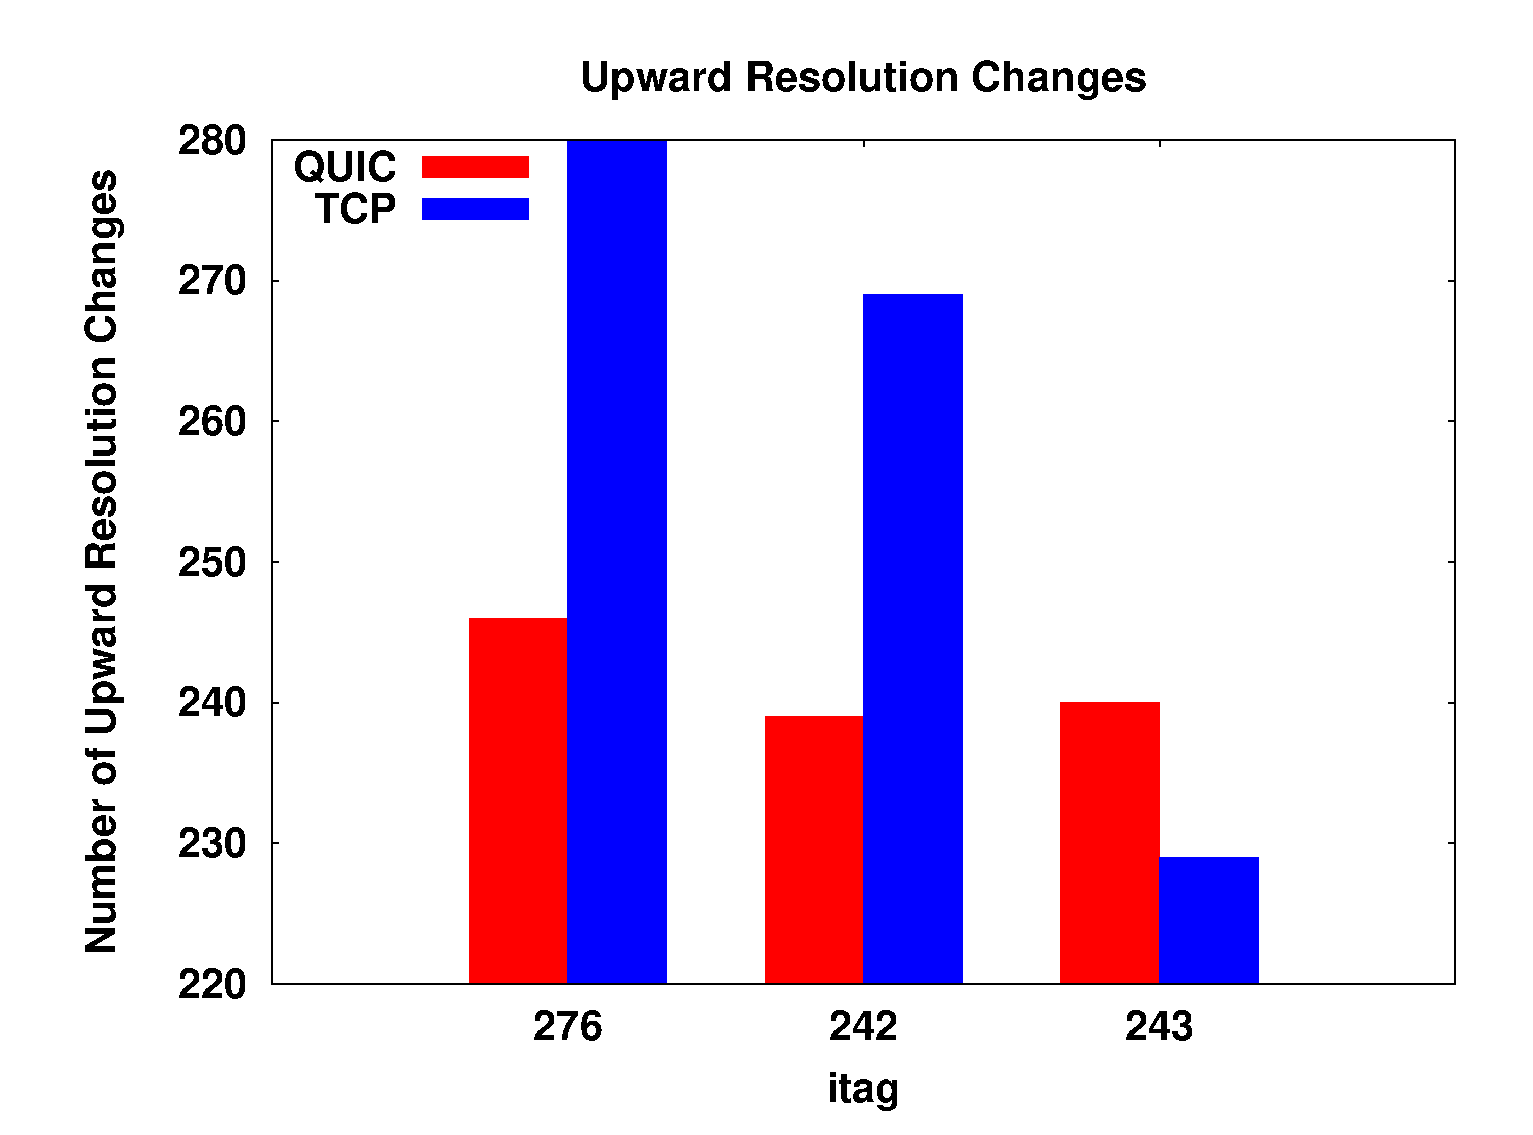
\includegraphics[width=\linewidth]{img/CDF/Data_up} 
\caption{Plot for Upward Resolution Changes}
\label{fig:clean11Q}
\end{minipage}
\begin{minipage}{0.48\linewidth}
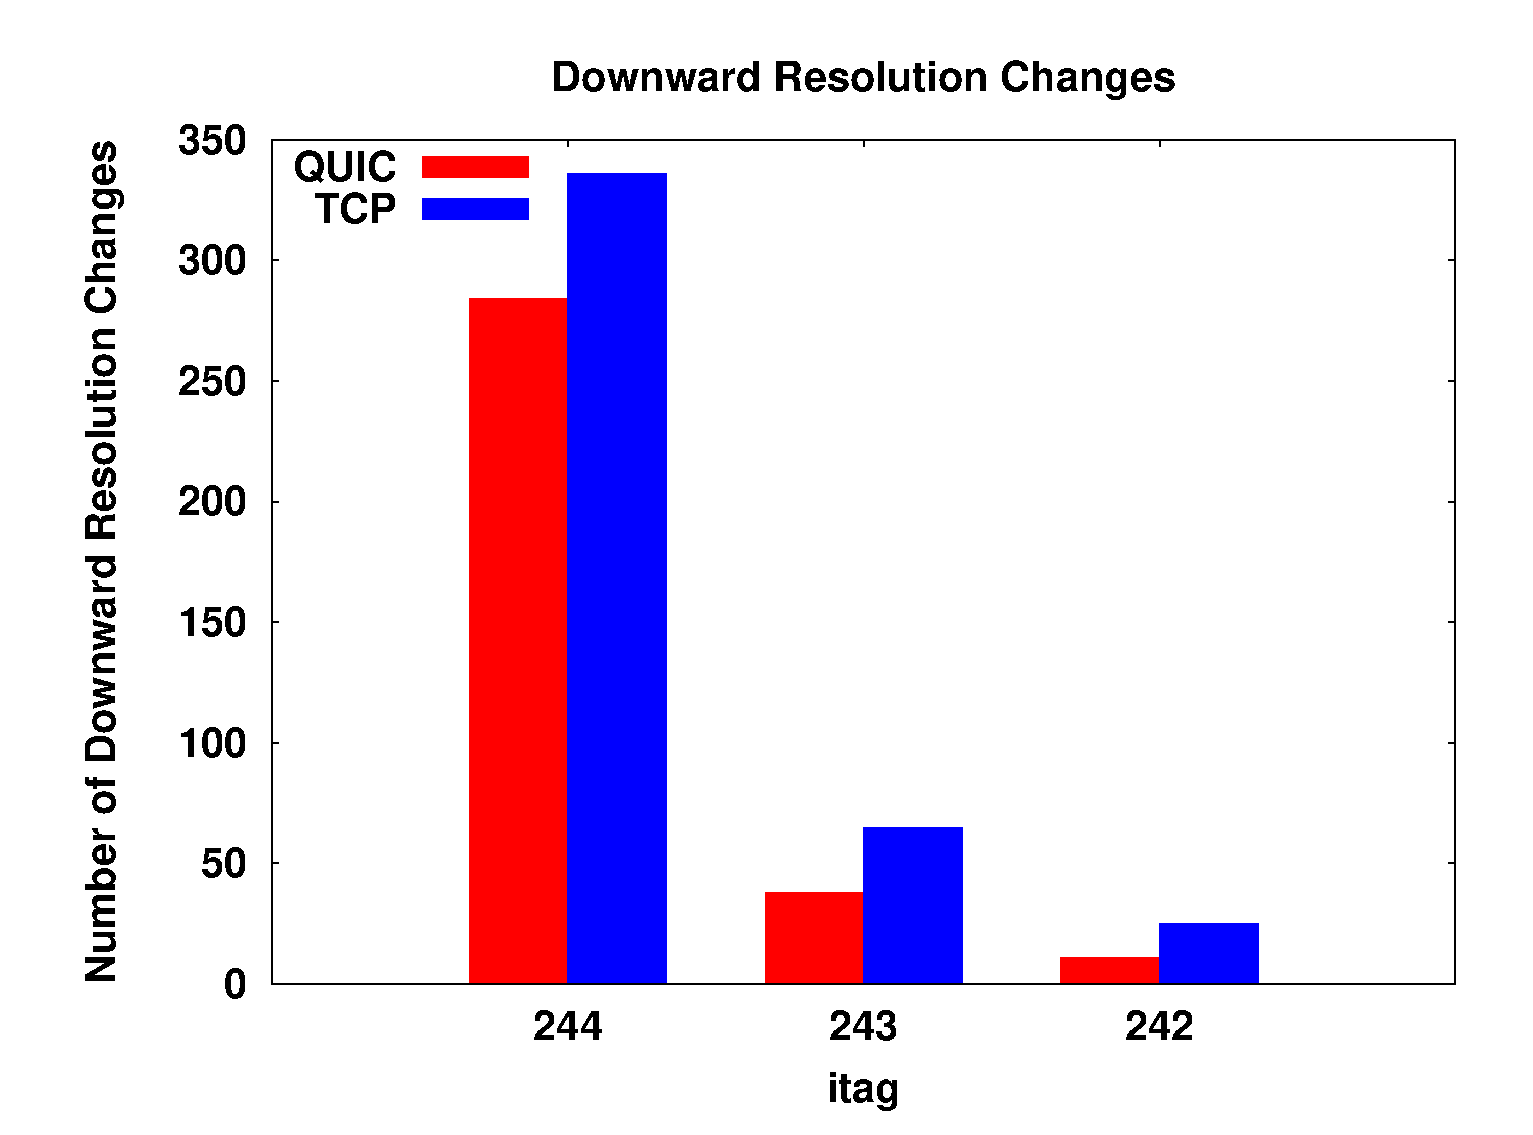
\includegraphics[width=\linewidth]{img/CDF/Data_down}
\caption{Plot for Downward Resolution Changes}
\label{fig:clen11T}
\end{minipage} 
\caption{Plot for Number of times Video Resolution Changed }
\label{fig:claen1}
\end{figure}



